%TC:envir minted 1 xall 
%TC:envir algorithmic 1 xall

% Include tables in word count
%TC:envir table 0 word
%TC:envir tabular 1 word

% Include footnotes in word count
%TC:macro \footnote [text]
%TC:macro \footnotetext [text]

%TC:group minted 0 0
%TC:macro \mintinline [ignore]
%TC:macro \colb [ignore]
%TC:macro \hyperref [ignore]

You will need three Raspberry Pis: two acting as hosts and one as the router. You will also need two Ethernet cables and two USB-to-Ethernet adapters. Use the cables to connect both your hosts to the router as shown below.

\begin{figure}[htbp]
  \centering
    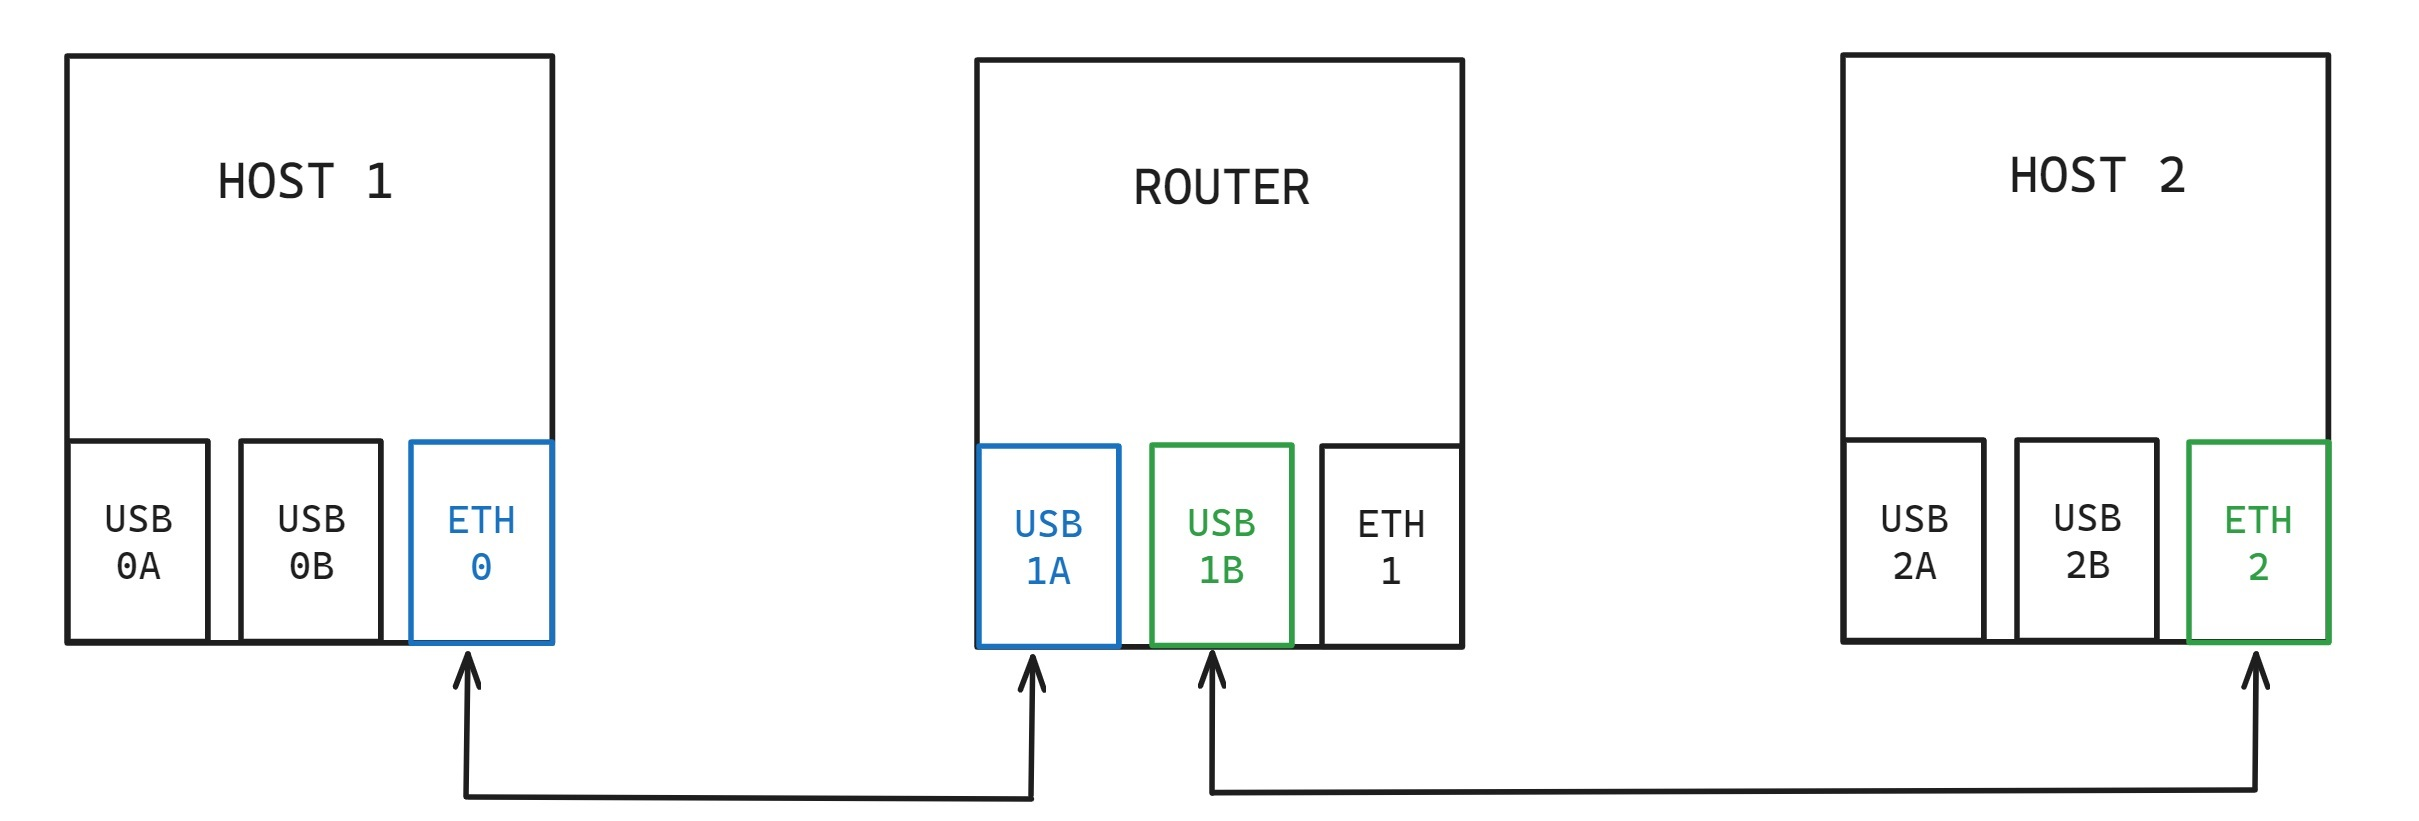
\includegraphics[width=1\textwidth]{figures/appendices/ipv6_setup.jpg}
\end{figure}

Run \texttt{ip a} on the router to learn the MAC and IP addresses of the two USB ports. Choose IPv6 addresses for the hosts such that they are on the same subnet as their corresponding router USB port. Let \texttt{IPa} and \texttt{IPb} denote the chosen IPv6 addresses for Host 1 and Host 2, respectively. On each host, run \texttt{ip a} to learn the MAC address of the host, henceforth referred to as \texttt{MACa} and \texttt{MACb}.

On Host 1, open a command prompt and run:
\begin{quote}
    \texttt{sudo ifconfig eth0 inet6 add IPa}
    
    \texttt{sudo ip -6 route add dev eth0 IPb}
    
    \texttt{sudo ip -6 neigh add dev eth0 IPb lladdr MACb}
\end{quote}

The first line sets a static IPv6 address for Host 1, the second line defines a route to Host 2 and the third line puts an entry in Host 1’s neighbour table, associating Host 2 with a specific MAC address.

Perform the same commands on Host 2:
\begin{quote}
    \texttt{sudo ifconfig eth0 inet6 add IPb}
    
    \texttt{sudo ip -6 route add dev eth0 IPa}
    
    \texttt{sudo ip -6 neigh add dev eth0 IPa lladdr MACa}
\end{quote}

Start the P4 program on the router and, using the CLI (or by using a \texttt{commands.txt} file, as explained in Appendix A), enter the commands:
\begin{quote}
    \texttt{table\_add MyIngress.ipv6\_lpm MyIngress.forward IPa/128 => MACa 0}
    
    \texttt{table\_add MyIngress.ipv6\_lpm MyIngress.forward IPb/128 => MACb 1}
\end{quote}

The \texttt{/128} network identifier prefix tells the router to only forward packets whose destination address matches exactly. This value can be changed to instruct the router to forward packets whose IPv6 address matches to any chosen bit size (i.e. perform a fixed-size prefix match, which can be extended to a longest prefix match).

On Host 1, run the command to send an Echo Request to Host 2:
\begin{quote}
    \texttt{ping6 -I eth0 IPb}
\end{quote}

Host 1 should be receiving Echo Replies from Host 2.